\documentclass[12pt,a4paper,titlepage,headinclude,bibtotoc]{scrartcl}

%---- Allgemeine Layout Einstellungen ------------------------------------------

% Für Kopf und Fußzeilen, siehe auch KOMA-Skript Doku
\usepackage[komastyle]{scrpage2}
\pagestyle{plain}
\setheadsepline{0.5pt}[\color{black}]
\automark[section]{chapter}


%Einstellungen für Figuren- und Tabellenbeschriftungen
\setkomafont{captionlabel}{\sffamily\bfseries}
\setcapindent{0em}


%---- Weitere Pakete -----------------------------------------------------------
% Die Pakete sind alle in der TeX Live Distribution enthalten. Wichtige Adressen
% www.ctan.org, www.dante.de

% Sprachunterstützung
\usepackage[ngerman]{babel}

% Benutzung von Umlauten direkt im Text
% entweder "latin1" oder "utf8"
\usepackage[utf8]{inputenc}

% Pakete mit Mathesymbolen und zur Beseitigung von Schwächen der Mathe-Umgebung
\usepackage{latexsym,exscale,stmaryrd,amssymb,amsmath}


\usepackage[nointegrals]{wasysym}
\usepackage{eurosym}

% Anderes Literaturverzeichnisformat
%\usepackage[square,sort&compress]{natbib}
\usepackage{hyperref}
% Für Farbe
\usepackage{color}
\usepackage{graphicx}
\usepackage{wrapfig}
\usepackage{subfigure}

% Caption neben Abbildung
\usepackage{sidecap}

% Befehl für "Entspricht"-Zeichen
\newcommand{\corresponds}{\ensuremath{\mathrel{\widehat{=}}}}
% Befehl für Errorfunction
\newcommand{\erf}[1]{\text{ erf}\ensuremath{\left( #1 \right)}}

%Fußnoten zwingend auf diese Seite setzen
\interfootnotelinepenalty=1000

%Für chemische Formeln (von www.dante.de)
%% Anpassung an LaTeX(2e) von Bernd Raichle
\makeatletter
\DeclareRobustCommand{\chemical}[1]{%
  {\(\m@th
   \edef\resetfontdimens{\noexpand\)%
       \fontdimen16\textfont2=\the\fontdimen16\textfont2
       \fontdimen17\textfont2=\the\fontdimen17\textfont2\relax}%
   \fontdimen16\textfont2=2.7pt \fontdimen17\textfont2=2.7pt
   \mathrm{#1}%
   \resetfontdimens}}
\makeatother

%Honecker-Kasten mit $$\shadowbox{$xxxx$}$$
\usepackage{fancybox}

%SI-Package
\usepackage{siunitx}

%keine Einrückung, wenn Latex doppelte Leerzeile
\parindent0pt

%Bibliography \bibliography{literatur} und \cite{gerthsen}
%\usepackage{cite}
\usepackage{babelbib}
\selectbiblanguage{ngerman}

\begin{document}

\begin{titlepage}
\centering
\textsc{\Large Praktikum zur Einführung in die physikalische Chemie,\\[1.5ex] Universität Göttingen}

\vspace*{1cm}

\rule{\textwidth}{1pt}\\[0.5cm]
{\huge \bfseries
  V6: Dissoziationskonstante\\[1.5ex]
  einer schwachen Säure}\\[0.5cm]
\rule{\textwidth}{1pt}

\vspace*{3cm}


\begin{Large}
\begin{tabular}{ll}
Durchführende: &  Alea Tokita, Julia Stachowiak\\
Assistentin: & Annemarie Kehl\\
 Versuchsdatum: & 18.01.2016\\
 Datum der Abgabe: & 25.01.2016\\
\end{tabular}
\end{Large}

\vspace*{1cm}

\begin{Large}
\fbox{
  \begin{minipage}[t][5cm][t]{5cm} 
  \textbf{Werte:}\\
  \end{minipage}
}
\end{Large}

\end{titlepage}

\tableofcontents

\newpage

\section{Theoretische Grundlagen}

Die Dissoziationskonstante der schwachen Säure p-Nitrophenol soll mittels Photometrie gemessen werden. \\
Säuren bilden in wässriger Lösung folgendes Gleichgewicht; $\mathrm{A^-}$ beschreibt den Säurerest.\\

\begin{equation}
\mathrm{HA}  \rightleftharpoons \mathrm{H^+} + \mathrm{A^-}
\end{equation}

Die Lage des Gleichgewichtes ist durch das Massenwirkungsgesetz definiert:\\

\begin{equation}
K_\mathrm{c} =\frac{c(\mathrm{H+}*c{A^-}{c(HA)}
\end{equation}

Der $\mathrm{pK_s}$-Wert ist der negativ dekadische Logarithmus von $\mathrm{K_S}$; der PH-Wert der negativ dekadische Logarithmus der Oxoniumionenkonzentration:

\begin{equation}
\mathrm{p}K_\mathrm{S} = - log_{10} (\frac{c(H^+}{c^0}
\end{equation}

\begin{equation}
\mathrm{PH}= -log_{10}(\frac{c(H^+)}{c^0})
\end{equation}

$c^0$ bezeichnet die Standartkonzentration von 1 $mol\cdot l^{-1}$ und wird verwandt, um den Term einheitenlos zu machen.


Gesucht wird somit nun $\mathrm{c(R^-)}$, da dies für die Abschwächung der Lichtintensität verantwortlich ist. Eine Pufferlösung gibt den PH-Wert vor. Bei Zugabe von einer Säure ändert sich dieser nur schwach und kann mittels der Henderson- Hasselbalch- Gleichung bestimmt werden: \\

\begin{equation}
pH = \mathrm{PK_S} + log_{10}\left(\frac{c(A^-}{c(HA)}
\end{equation}

$\mathrm{c(A^-}$ und $\mathrm{c(HA)}$ beschreibt die Konzentrationen des Puffers im Gleichgewicht. \\

\subsection{Photometrie}
Die Verminderung der Lichtintensität $\mathrm{d}I$ der Lösung im Vergleich zu der Lichtintensität von Wasser $I_0$, ist ein Maß für die Konzentration der absorbierenden Substanz. Sie wird über den Weg $x$, hier gleichzusetzen mit der Küvettenschichtdicke $d$. Sie wird durch das Lambert-Beersche Gesetz beschrieben ergibt die Extinktion $E$:\\

\begin{equation}
E = \epsilon_\lambda \cdot c \cdot d = log_{10}\left(\frac{I_0}{I}
\end{equation}

$\epsilon_lambda$ beschreibt die Extinktionskonstante. 








%\begin{equation}
-\frac{\mathrm{d}I}{\mathrm{d}x} = \alpha \cdot c(A^-) \cdot I
\end{equation}








Henderson-Hasselbalch-Gleichung, Pufferlösung und schwache Säure???








In Lösung bildet p-Nitrophenol folgendes Gleichgewicht:










\centering
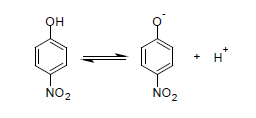
\includegraphics[scale=1]{Strukturformel}

Die dissoziierte und undissoziierte Form weisen eine unterschiedliche Lichtdurchlässigkeit auf.
Bei Auftreffen von Licht klappt die eine Ladung der dissoziierten Form herunter etc. und somit ist die dissoziierte Form gelb und dadurch lichtundurchlässiger als die dissoziierte Form.


\section{Bestimmung der Dissoziationskonstante}




\subsection{Versuchsaufbau}
+ Versuchsaufbau; Photometer

\subsection{Durchführung}




\section{Auswertung}
Im Versuch wird die Messung der Extinktion für jeden pH, sowie für $E_{\infty}$, sechsmal durchgeführt. Anschließend wird daraus für jeden pH der Mittelwert der Extinktion gebildet. Es ergeben sich folgende Mittelwerte:

\begin{table} [h]
\begin{tabular} {| p {1,5 cm}|| p {3 cm}|}
  \hline\\
  pH & $\overline{E}$\\\hline
  $6,2$& $0,18$\\\hline
  $6,4$& $0,255$\\\hline
  $6,6$& $0,347$\\\hline
  $6,8$& $0,463$\\\hline
  $7,0$& $0,659$\\\hline
  $7,2$& $0,827$\\\hline
  $7,4$& $0,948$\\\hline
  $7,6$& $1,044$\\\hline
 

\end{tabular}
\end{table}
Für   
\end{document}
